\begin{center}

  \begin{tabular}{rp{16cm}lp{20cm}}%{rl}

  % after \\: \hline or \cline{col1-col2} \cline{col3-col4} ...

  论文地址:& \href{https://arxiv.org/pdf/1902.10191}{https://arxiv.org/pdf/1902.10191} \\
  来源:& AAAI, 2020 \\
  作者:& Pareja, Aldo, et al. \\
  源码:& \href{https://github.com/IBM/EvolveGCN}{EvolveGCN} \\

%  slides:& \href{http://yunshengb.com/wp-content/uploads/2017/03/nips_2018_r2l_workshop_talk.pdf}{{\footnotesize Convolutional Set Matching for Graph Similarity}}\\

  关键词:& \textbf{Dynamic Graphs, GCN} \\

  写于:& \date{2021-02-17}

  \end{tabular}

\end{center}

该论文\cite{pareja2019evolvegcn}解决的是不断进化(evolve)的graph的表征问题。以往的方法主要将结点的表征通过RNN来学习不断进化的graph,这种方法在学习表征时需要知道结点在所有时间区间上的变化(相当于是transductive的),并且在变化比较频繁的graph上不太友好。论文提出EvolveGCN,将GCN和RNN结合,使用RNN来学习GCN的参数,以此来捕捉动态图的动态性。

\paragraph{问题定义}
对于一个动态图$G$,在每一个时间点$t$上,可以将$G$表示为$(A_t,X_t)$,分别表示时间$t$时的邻接矩阵和特征矩阵。最终要学习的是$G$中每个结点在各个时间点上的结点表征。

\begin{figure}[h]
	\centering
	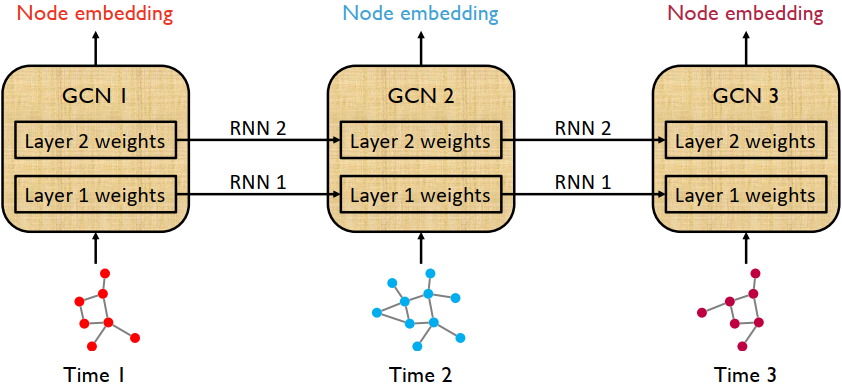
\includegraphics[width=.8\textwidth]{pics/EvolveGCN.png}
	\caption{EvolveGCN}
	\label{fig:evolvegcn}
\end{figure}

\paragraph{EvolveGCN思路}
如Fig.\ref{fig:evolvegcn}所示,在时间点$t$时,将$(A_t,X_t)$输入到模型中,可以学习到$t$时的结点表征。注意,\tbc{red}{GCN的参数并不是训练得来的,而是通过RNN计算得到的}。GCN在EvolveGCN中起的作用:通过$(A_t,X_t)$得到结点表征,但是并不会在计算表征的过程中更新GCN各层的参数。RNN在EvolveGCN中起的作用:在$t-1$时的结点表征和GCN参数的基础上更新GCN的参数,更新公式如下:
$$
\overbrace{\underbrace{W_{t}^{(l)}}_{\text {hidden state }}}^{\text {GCN weights }}=\operatorname{GRU}(\underbrace{\overbrace{H_{t}^{(l)}}^{\text {node embeddings }}}_{\text {input }}, \overbrace{\underbrace{W_{t-1}^{(l)}}_{\text {hidden state }}}^{\text {GCN weights }})
$$
或
$$
\overbrace{\underbrace{W_{t}^{(l)}}^{\text {GCN weights }}}_{\text {output }}=\operatorname{LSTM}(\overbrace{\underbrace{W_{t-1}^{(l)}}_{\text {input }}}^{\text {GCN weights }})
$$
从上可以得到,动态图的变化都保存在了GCN的参数中。在实现时,需要对RNN进行更改:
\begin{itemize}
	\item 将RNN单元的输入与隐状态扩展为矩阵形式,因为GCN的参数和结点表征都是矩阵的形式
	\item 将输入的列与隐状态的列相匹配
\end{itemize}


\paragraph{方法解决的问题/优势}
\begin{itemize}

	\item 对动态图的表征学习提出了可行的解决方法
	\item 将RNN和GCN相结合,利用RNN来进化GCN的参数,能够应对变化频繁的graph,而且不需要提前预知结点的所有变化

\end{itemize}


\paragraph{方法的局限性/未来方向}

\begin{itemize}
	\item 虽然不需要提前预知结点的所有变化,但是\tbc{red}{需要预知graph中的所有结点,不能应对结点的变化}
	\item 使用RNN来进化GCN的参数,将graph的动态性保存在参数中,一个训练好的模型也许只能捕捉一种动态性

\end{itemize}



